\documentclass{article}
\usepackage{amsmath,amssymb,amsthm,fullpage,enumerate,hyperref,graphicx}
\usepackage[color]{changebar}
\cbcolor{blue}
\theoremstyle{definition}
\newtheorem{defi}{Definition}
\newtheorem{theo}{Theorem}
\newtheorem{prop}{Proposition}
\newtheorem{claim}{Claim}
\begin{document}
\section{Starting point}
We take a lattice
\[L=\mathbb{Z}\omega_1+\mathbb{Z}\omega_2,\]
for some $\omega_1,\omega_2\in\mathbb{C}$ not on the same line. Then $\mathbb{C}/L$ is topologically a torus.

Since we're going to do differential geometry, we want to find an explicit map. We recall that the origin-centered torus is given parametrically as
\begin{align*}
  x(\theta,\phi)&=(R+r\cos(\theta))\cos(\phi)\\
  y(\theta,\phi)&=(R+r\cos(\theta))\sin(\phi)\\
  z(\theta,\phi)&=r\sin(\theta),
\end{align*}
where $0\leq\theta,\phi\leq 2\pi$ and $R$ is the distance from the center of the tube to the center of the torus, and $r$ is the radius of the tube. We denote this torus by $\mathbb{T}^2(R,r)$. If you plot $\mathbb{T}^2(R,r)$ you'll notice that $\theta$ specifies angle in relation to the center of the tube, and $\phi$ specifies angle in relation to the center of the torus. As in the below picture:

\begin{figure}[h]
  \centering
  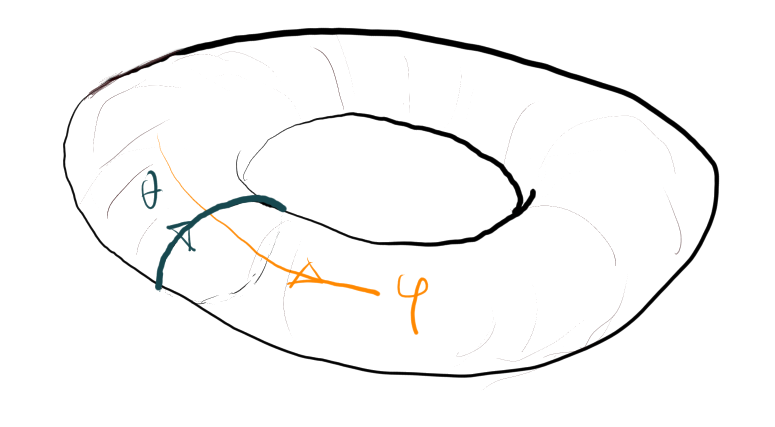
\includegraphics[width=0.6\textwidth]{theta_phi.png}
\end{figure}

To figure out the map from $\mathbb{C}/L$ to $\mathbb{T}^2(R,r)$ we essentially just have to figure out how to map a point on the ``parallellogram with sides identified'' to a point on $\mathbb{T}^2(R,r)$ for some appropriate $R$ and $r$.

There are several ways of doing this, and here's but one. Let $F:\mathbb{C}\to\mathbb{T}^2(1,1)$ be given by
\[F(\alpha\omega_1+\beta\omega_2)=(x,y,z)(\alpha\cdot2\pi,\beta\cdot2\pi).\]
Since $\omega_1$ and $\omega_2$ are linearly independent, this is well-defined, and since $\cos$ and $\sin$ are $2\pi$-periodic, $F$ descends to a function $\tilde{F}:\mathbb{C}/L\to\mathbb{T}^2(R,r)$. It is clear that viewed as function from $\mathbb{R}^2$ to $\mathbb{R}^3$, $F$ is a diffeomorphism.

By the way, I'm making the gentle assumption that $\omega_1$ and $\omega_2$ are both in the first quadrant.

Excellent, so let's now bring in some definitions from Spivak so that we can make sense of $\mathrm{d}z$ -- the translation invariant one-form.
\section{Definitions from Spivak}
We begin with a $k$-dimensional manifold.
\begin{defi}
  A subset $M\subseteq\mathbb{R}^n$ is called a $k$-dimensional manifold if for
  every $x\in M$ it holds that
  \begin{quotation}
    there exists an open set $U\ni x$ and an open set $V\subseteq\mathbb{R}^n$ and
    a diffeomorphism $h:U\to V$ such that
    \[h(U\cap M)=V\cap(\mathbb{R}^k\times\{\mathbf{0}\}).\]
  \end{quotation}
\end{defi}
To see that $\mathbb{T}^2(R,r)$ is a $2$-manifold, we have to think a little bit. Take $v\in M$ arbitrary, say with $v=(x(\theta',\phi'),y(\theta',\phi),z(\theta',\phi'))$ with $0\leq\theta',\phi<2\pi$. Let $0\leq\epsilon<\pi/4$ be arbitrary and put
\[P=\{(x(\theta'+2\pi\delta_{\theta',0}+s,\phi'+t),y(\theta'+2\pi\delta_{\theta',0}+s,\phi'+t),z(\theta'+2\pi\delta_{\theta',0}+s,\phi'+t)):-\epsilon<s,t<\epsilon\}.\]
Here $P$ stands for ``patch''. Let
\[w=(x(\pi/2,\phi'),y(\pi/2,\phi'),z(\pi/2,\phi')),\]
and let
\[U=\{p+rw:p\in P,-1/2<r<1/2\}.\]
Hence $U\cap M=P$. I take as geometrically clear that $U$ is indeed an open set. Let now
\[V=\{(s,t,u):-\epsilon<s,t<\epsilon,-1/2<u<1/2\},\]
and define $h:U\to V$ by
\[h(x(\theta'+2\pi\delta_{\theta',0}+s,\phi'+t)+rw_1,y(\theta'+2\pi\delta_{\theta',0}+s,\phi'+t)+rw_2,z(\theta'+2\pi\delta_{\theta',0}+s,\phi'+t)+rw_3)=(s,t,r).\]
Since any point in in $U$ is determined uniquely by the parameters $s$, $t$, and $r$, we have that $h$ is well-defined, and some first year calculus shows that it's smooth.

We see that
\[h(U\cap M)=h(P)=\{(s,t,0):-\epsilon<s,t<\epsilon\}=V\cap\mathbb{R}^2\times\{0\},\]
and so we conclude that $\mathbb{T}^2(R,r)$ indeed is a $2$-manifold.

I will take the view that $\mathbb{C}/L$ is simply identified with $\mathbb{T}^2(1,1)$ through $\tilde{F}$. This is because Spivak doesn't include an ambient space. {\tt Frankly, when giving the talk I will probably just use Lee's ``Smooth Manifolds'' instead or better yet Wells' ``Differential Analysis on Complex Manifolds'' because it's a bit difficult to translate notions all the time. On the other hand, Wells' and Lee kind of go off the deep end into some algebraic geometry. So there's that.}

Before continuing to {\it forms}, let's talk about coordinate systems. Spivak gives the following theorem.
\begin{theo}
  A subset $M$ of $\mathbb{R}^n$ is a $k$-dimensional manifold iff for every $x\in M$ the following condition is satisfied:
  \begin{quotation}
    There is an open set $U\ni x$ and an open set $W\subseteq\mathbb{R}^k$ and an injective smooth function $f:W\to\mathbb{R}^n$ such that
    \begin{enumerate}
      \item $f(W)=M\cap U$,
      \item $f'(y)$ has rank $k$ for every $y\in W$,
      \item $f^{-1}:f(W)\to W$ is continuous.
    \end{enumerate}
  \end{quotation}
  Such a function $f$ is called a coordinate system around $x$.
\end{theo}
I'm pretty sure that in modern terminology -- this corresponds to having an atlas.
\section{Forms}
Before we treat forms on manifolds, we need to recall what forms are in Euclidean space. For this, we need the concept of tensors, alternating tensors, and the wedge product. From Spivak's point of view, this isn't too bad. {\tt Although he seems to consciously skip the concept of vector and tangent bundles, which makes it a bit harder to define things.}

Let's start with tensors.
\begin{defi}[Tensor]
  Let $V$ be an $\mathbb{R}$-vector space, and let $k$ be a positive integer. Then a $k$-tensor on $V$ is a multilinear function $T:V^k\to\mathbb{R}$. The set of all $k$-tensors on $V$ is denoted by $\mathcal{T}^k(V)$. It forms a vector space given
  \[(S+T)(v)=S(v)+T(v),\]
  and
  \[(rS)(v)=rS(v),\]
  for $S,T\in\mathcal{T}^k(V)$ and $r\in\mathbb{R}$ and $v\in V$.
\end{defi}
In other words, $\mathcal{T}^k(V)=(V^k)^\vee$. If $T\in\mathcal{T}^k(V)$ it's called {\it alternating} if
\[T(v_1,\dots,v_i,\dots,v_j,\dots,v_k)=-T(v_1,\dots,v_j,\dots,v_i,\dots,v_k),\]
for any $i<j$. The space of all alternating $k$-tensors on $V$ is denoted by $\Lambda^k(V)$.

In this setting, the tensor product $\otimes$ is defined as follows.
\begin{defi}
  Let $V$ be an $\mathbb{R}$-vector space. Let $S\in\mathcal{T}^k(V)$ and $T\in\mathcal{T}^l(V)$. Then we define
  \[(S\otimes T)(v_1,\dots,v_k,v_{k+1},\dots,v_{k+l})=S(v_1,\dots,v_k)T(v_{k+1},\dots,v_{k+l}),\]
  and notice $S\otimes T\in\mathcal{T}^{k+l}(V)$.
\end{defi}
We can construct alternating tensors from tensors using the $\mathrm{Alt}$-map, defined as follows. Let $T\in\mathcal{T}^k(V)$, then put
\[\mathrm{Alt}(T)(v)=\frac{1}{k!}\sum_{\sigma\in S_k}\mathrm{sgn}(\sigma)T(\sigma.v),\]
where $\sigma$ acts by permutating the canonical basis. Clearly $\mathrm{Alt}$ is a generalization of the determinant.

It's a fact that if $T\in\mathcal{T}^k(V)$ then $\mathrm{Alt}(T)\in\Lambda^k(V)$ and $\mathrm{Alt}(\mathrm{Alt}(T))=T$, and if $\omega\in\Lambda^k(V)$, then $\mathrm{Alt}(\omega)=\omega$.

We can form products also on the space of alternating tensors.
\begin{defi}[Wedge product]
  Let $\omega\in\Lambda^k(V)$ and $\eta\in\Lambda^l(V)$ for some $\mathbb{R}$-vector space. Then we define
  \[\omega\land\eta=\frac{(k+l)!}{k!l!}\mathrm{Alt}(\omega\otimes\eta).\]
  It holds that $\omega\land\eta\in\Lambda^{k+l}(V)$.
\end{defi}
We can use the wedge product to get a basis for $\Lambda^k(V)$.
\begin{prop}
  Let $\{e_i\}_{i=1}^n$ be a basis for $V$. Then
  \[e_{i_1}^\vee\land\dots\land e_{i_k}^\vee,\]
  where $1\leq i_1<i_2<\dots<i_k\leq n$, forms a basis for $\Lambda^k(V)$.
\end{prop}

Now we're really close to defining forms. First we need the concept of a tangent space.
\begin{defi}[Tangent space]
  Let $n$ be a positive integer and let $p\in\mathbb{R}^n$. Then we define
  \[\mathbb{R}^n_p=\{(p,v):v\in\mathbb{R}^n\},\]
  and $(p,v)+(p,w)=(p,v+w)$ and $a(p,v)=(p,av)$. This turns $\mathbb{R}^n_p$ into a vector space, which we call the tangent space at $p$.

  We usually write $v_p$ for $(p,v)$.
\end{defi}
We will probably need the notion of vector fields, so I'll define that too.
\begin{defi}[Vector field]
  A vector field is a function
  \[F:\mathbb{R}^n\to\bigsqcup_{p\in\mathbb{R}^n}\mathbb{R}^n_p,\]
  such that $F(p)\in\mathbb{R}^n_p$ for every $p\in\mathbb{R}^n$.
\end{defi}
Notice that $(e_i)_p$ is a basis for $\mathbb{R}^n_p$, and thus we have
\[F(p)=\sum_{i=1}^nF^i(p)(e_i)_p,\]
for some component functions $F^i$. We call $F$ continuous or smooth if the $F^i$ are continuous or smooth; respectively.

And here we go, now we can define a differential form.
\begin{defi}[Differential form]
  A differential $k$-form on $\mathbb{R}^n$ is a function $\omega:\mathbb{R}^n\to\bigsqcup_{p\in\mathbb{R}^n}\Lambda^k(\mathbb{R}^n_p)$ with $\omega(p)\in\Lambda^k(\mathbb{R}^n_p)$.
\end{defi}
Since we know a basis for $\Lambda^k(V)$, we see that any $k$-form $\omega$ can be written as
\[\omega(p)=\sum_{1\leq i_1<\dots<i_k\leq n}\omega_{i_1,\dots,i_k}(p)\phi_{i_1}(p)\land\dots\land\phi_{i_k}(p),\]
for some coefficients $\omega_{i_1,\dots,i_k}(p)\in\mathbb{R}$, and $\phi_i=(e_i)_p^\vee$.

If the coefficient functions $p\mapsto\omega_{i_1,\dots,i_k}(p)$ are continuous or smooth, then we call the $k$-form $\omega$ continuous, or smooth; respectively.

Suppose now that $f:\mathbb{R}^n\to\mathbb{R}$ is smooth.
\begin{claim}
  Then $Df(p)\in\Lambda^1(\mathbb{R}^n)$.
\end{claim}
\begin{proof}
  By definition $Df(p)=\lambda:\mathbb{R}^n\to\mathbb{R}$ is the unique linear transformation satisfying
  \[\lim_{h\to 0}|f(p+h)-f(h)-\lambda(h)|/|h|=0.\]
  So $\lambda$, because it's linear, is a $1$-tensor. But then it's alternating (vacuously).
\end{proof}
Using this, we can define $df$, for $f:\mathbb{R}^n\to\mathbb{R}$ smooth.
\begin{defi}
  Let $f:\mathbb{R}^n\to\mathbb{R}$ be smooth. Then we define $df:\mathbb{R}^n\to\bigsqcup_{p\in\mathbb{R}^n}\Lambda^1(\mathbb{R}^n_p)$ by
  \[df(p)(v_p)=Df(p)(v).\]
\end{defi}
Let in particular $\pi^i:\mathbb{R}^n\to\mathbb{R}$ be defined by $\pi^i(x)=x^i$. Notice now that
\[d\pi^i(p)(v_p)=D\pi^i(p)(v)=e_i^Tv=v^i,\]
So $d\pi^i(p)((e_j)_p)=[i=j]$, so $d\pi^i(p)=(e_i)_p^\vee$. Usually we write $x^i$ for $\pi^i$, and thus any differential $k$-form can be written as
\[\omega(p)=\sum_{1\leq i_1<\dots<i_k\leq n}\omega_{i_1,\dots,i_k}(p)dx^{i_1}\land\dots\land dx^{i_k}.\]
When defining differential forms on manifolds, we want to induce smooth functions $\mathbb{R}^n\to\mathbb{R}^m$ to linear transformations $\mathbb{R}^n_p\to\mathbb{R}^n_{f(p)}$. This is how we do it.
\begin{defi}
  Let $f:\mathbb{R}^n\to\mathbb{R}^m$ be a smooth. Then we define $f_\ast:\mathbb{R}^n_p\to\mathbb{R}^m_{f(p)}$ by
  \[f_\ast(v_p)=(Df(p)(v))_{f(p)}.\]
\end{defi}
\begin{claim}
  It makes sense.
\end{claim}
\begin{proof}
  We have that $Df(p)$ is a linear transformation $\mathbb{R}^n\to\mathbb{R}^m$, so $Df(p)(v)\in\mathbb{R}^m$ and thus $(Df(p)(v))_{f(p)}$. Linearity should be fine.
\end{proof}
From $f_\ast$ we can induce further, to get a transformation
\[f^\ast:\Lambda^k(\mathbb{R}^m_{f(p)})\to\Lambda^k(\mathbb{R}^n_p),\]
in the usual way -- that is:
\[f^\ast(\omega)=\omega\circ f_\ast.\]
\begin{claim}
  This also makes sense.
\end{claim}
\begin{proof}
  Take $v_p\in\mathbb{R}^n_p$, then $f_\ast(v_p)\in\mathbb{R}^m_{f(p)}$, so is in the domain of $\omega$. Cool, we're fine.
\end{proof}
That's all we need for forms. So let's go to {\Huge\tt manifold town!}
\section{Forms on manifolds}
Let $M$ be a $k$-dimensional in $\mathbb{R}^n$ and let $f:W\to\mathbb{R}^n$ be a coordinate system around $x=f(a)$.
\begin{claim}
  It holds that $f_\ast:\mathbb{R}^k_a\to\mathbb{R}^n_x$ is injective, and $f_\ast(\mathbb{R}^k_a)$ is $k$-dimensional subspace of $\mathbb{R}^n_x$.
\end{claim}
\begin{proof}
  We have that $f_\ast(v_a)=(Df(a)(v))_x$. Since $f'(a)$ has rank $k$, the linear transformation $Df(a):W\to\mathbb{R}^k$ is an isomorphism. Therefore, $(Df(a)(v))_x=0$ implies $Df(a)(v)=0$ implies $v=0$ implies $v_a=0$. So also $f_\ast$ is injective.

  It's not surjective, but at least $f_\ast(\mathbb{R}^k_a)$ is an isomorphic copy of $\mathbb{R}^k_a$, so it is of dimension $k$.
\end{proof}
Let $g:V\to\mathbb{R}^n$ be any other coordinate system around $x=g(b)$. {\tt We assume, I think WLOG, that the $U\ni x$ is the same for both.}
\begin{claim}
  Its range is the same.
\end{claim}
\begin{proof}
  \cbstart
  Let's first prove that $g_\ast=f_\ast\circ(f^{-1}\circ g)_\ast$. This follows basically by the chain rule. Note that
  \[f^{-1}(g(b))=f^{-1}(x)=a,\]
  and therefore
  \[Df(a)D(f^{-1}\circ g)(b)=Df(f^{-1}(g(b)))D(f^{-1}\circ g)(b)=D(f\circ(f^{-1}\circ g))(b)=Dg(b).\]
  This means that
  \[f_\ast(f^{-1}\circ g)_\ast(v_b)=f_\ast((D(f^{-1}\circ g)(b)v)_a)=(Df(a)(D(f^{-1}\circ g)(b)v))_x=(Dg(b)v)_x=g_\ast(v_b).\]
  Let's now take a peek at
  \[(f^{-1}\circ g)_\ast(\mathbb{R}^k_b).\]
  We have that
  \[(f^{-1}\circ g)_\ast(\mathbb{R}^k_b)=\{(Df^{-1}g(b)\circ Dg(b)v)_a:v\in\mathbb{R}^k\}.\]
  Since $Dg(b)$ has rank $k$, we have that $Dg(b)v$ spans a $k$-dimensional subspace of $\mathbb{R}^n$. Since $Df(a)$ has rank $k$, it should be the case that $Df^{-1}(g(b))$ (which exists because reasons) also has rank $k$, and thus $Df^{-1}(g(b))Dg(b)v$ should be $k$-dimensional, and thus $\mathbb{R}^k$ itself.
  \cbend

  {\tt BTW:} The correct way is to say that $(g^{-1}\circ f)_\ast$ is an inverse to $(f^{-1}\circ g)_\ast$. No smoothness needed!
\end{proof}
{\tt Fishy argument. I need to fix this.}

The best way to fix this is to just use Lee. But, I'll let it slide for now. Let's just assume that it works. {\tt Damn it!}

{\tt Found a fix in ``Comprehensive Introduction'' volume 1. Yes!}

If $f:W\to\mathbb{R}^n$ is a coordinate system. We write
\[M_x=f_\ast(\mathbb{R}^k_a),\]
and call this the tangent space of $M$ at $x$. We can now define a differential $p$-form.
\begin{defi}[Form on a manifold]
  Let $\omega:M\to\bigsqcup_{x\in M}\Lambda^p(M_x)$ satisfy $\omega(x)\in\Lambda^p(M_x)$ for every $x\in M$. Then we call $\omega$ a $p$-form on $M$.

  If $f:W\to\mathbb{R}^n$ is a coordinate system, then $f^\ast\omega$ is a $p$-form on $W$, and we say that $\omega$ is smooth if $f^\ast\omega$ is.
\end{defi}
Next Spivak claims we can write $\omega$ as
\[\omega=\sum_{1\leq i_1<\dots<i_p\leq n}\omega_{i_1,\dots,i_p}dx^{i_1}\land\dots\land dx^{i_p},\]
and this means we need to make sense of
\[dx^{i_j}(p),\]
for $p\in M$. Can we? Previously we defined it as
\[d\pi^i(v)(w\in M_x)=D\pi^i(v)(w),\]
but we probably need to use coordinate systems now.

And yes we do, but recall that $M_x=f_\ast(\mathbb{R}^k_a)$ actually sits inside $\mathbb{R}^n_x$, so we in fact use the same $d\pi^i$ as before.

But, when we want to carry over $dz$ to $\mathbb{T}^2$ we get a problem. It's the case that
\[f_\ast(\mathbb{R}^2_a)\subset\mathbb{R}^3_x,\]
so we can impossible make sense of $(dx,dy)$, because $dx$ and $dy$ only make sense in $\mathbb{R}^2_x$. Here's where our grand plan stops making sense.
\end{document}
